\section{Introduction}
\label{sec:intro}



\red{First draft of the intro. Flow: motivation and examples -> related works -> our approach -> contributions}

\begin{figure}[t]
\centering
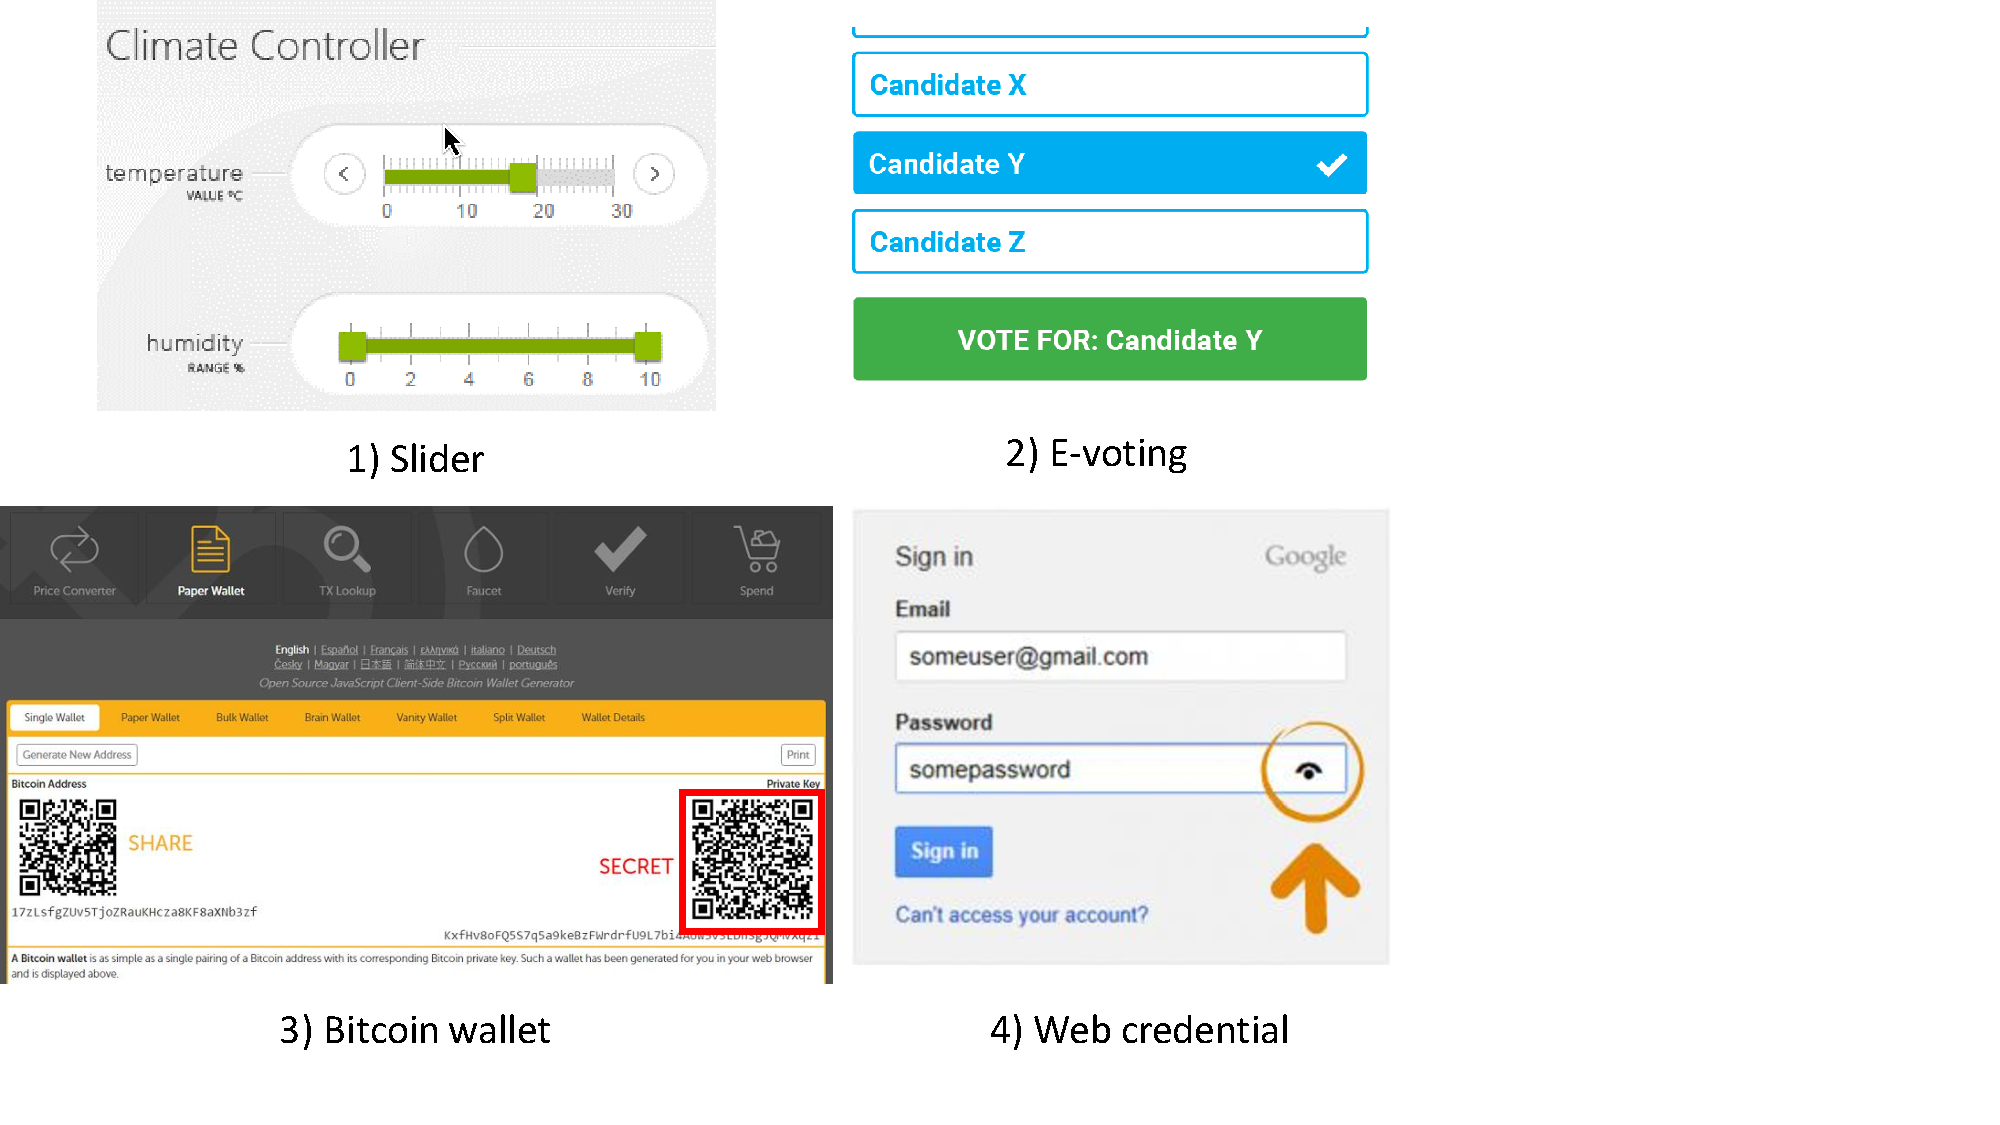
\includegraphics[trim={0 1cm 10cm 0}, clip, width=\linewidth]{motivation.pdf}
\caption{\textbf{Motivating examples.} 1) Pointer based UI elements that sets parameters to remote safety-critical device, 2) E-voting where the voting privacy and integrity is critical, 3) Financial transactions such as bitcoin wallet that shows sensitive information such as the user's private key and 4) web applications that provide an option for the user to reveal credentials.}
\spacesave
\label{fig:motivation}
\centering
\end{figure}

%Describe the overall problems with examples of attacks. Remote server, safety critical devices, credentials.
%The advancement of computer systems in the last two decades has transformed fundamentally the way end-users interact with remote service providers. In the same time, 
The complexity of modern operating systems and softwares has proven that computers largely remain vulnerable to attacks. A compromised computer threatens the integrity and the confidentiality of any interaction between the user and a remote server. It can easily alter the data transferred from the user to the remote server, or trick the user to perform unintended actions, or just observe any sensitive communication going through. Therefore, the necessity of trusted paths for IO between the user and remote servers is essential.

\texttt{Output Integrity.} Ensuring that the user performs intended actions to the remote server, typically, requires to assure that the user gets authentic output from the server. For example, a user configuring remotely a safety-critical device bases her inputs in the current state of the system. As illustrated in the Figure~\ref{fig:motivation}, a compromised host could trick the user to perform unintended actions by providing incorrect feedback about the actual status. \texttt{Output Confidentiality.} Other applications require that the trusted paths provide a mechanism for the remote server to show secret information to the user. Figure~\ref{fig:motivation} illustrates such cases when a web server delivers a private key of a crypto-wallet to the user which should be kept hidden to the untrusted host.

\texttt{Input Integrity.} Once that output security is achieved, the trusted paths should guarantee that the remote servers accepts only inputs generated by the honest user. This feature is critical for the integrity of user actions in case of a compromised host. As shown in Figure~\ref{fig:motivation}, the user submits her inputs and the remote server assures that a malicious host has not altered user's original inputs. \texttt{Input Confidentiality.} Other applications (e.g., e-voting) require a higher level of security, the inputs should be sent to the server as generated by the user---input integrity---and preferably the host should not have access to inputs. Note that, in order to provide input security, trusted paths should guarantee at first output security. \footnote{Is this a strong statement?}

Human interaction with computers is one of the most fundamental components in today's complex systems, and interfaces are crucial for the interactions. All computing devices, such as desktop computers, smartwatches, embedded devices provide some input mechanisms via the user interfaces (UI) where the users can provide input to the computers. These input interfaces are the embodiments of the human-computer interaction (HCI). Critical infrastructures and automation systems rely on human input, and the correctness of the input is of uttermost importance. Human interaction with the computer systems over the last few decades evolves both in diversity and complexity. This gives rise to a major threat concerning the integrity and the confidentiality of the user input. Recent revelations like Snowden leaks show that powerful attackers such as state nations can compromise general purpose computing systems (we call them \emph{host} systems, e.g., computers, smartphone, etc.) that include both operating systems and hardware. Research works such as A2~\cite{A2} shows the first fabrication-time attack that can leverage the space common to Application-Specific Integrated Circuit (ASIC) layouts to implement malicious circuits. Such attacks are major threats to the security and privacy of the user interaction with the system as the attacker can monitor and manipulate user interactions. 
Figure~\ref{fig:motivation} provides four such potential uses cases out of many, where the integrity and confidentiality of user IO data are critical. Networked safety-critical systems, such as Programmable Logic Controllers in a factory plant, are often remotely configurable by administrators through web-based interfaces. Other applications such as home automation systems, medical devices also expose their functionality through web APIs. Apart from the cyber-physical system, other web-based applications such as internet banking, user input are very critical. Manipulating user input in these applications could lead to catastrophic failures, even compromise the safety of humans. Hence, integrity is one of the major aspects while providing input parameters to a critical system. Apart from the integrity, the confidentiality of the user input is also of utmost importance for applications like e-voting, online messenger, web-service credentials, bitcoin wallet, etc. Secure transport layer protocols such as \https (or \tls) can be employed to secure the communication between the host system and the remote server, but the protocols assume that the host system is trusted which may not be the case provided the aforementioned attacker model.

InContext~\cite{huang2012clickjacking} presents different clickjacking attacks variants and their solution by ensuring context (both temporal and visual) and pointer integrity in the trusted browser setting. Trusted hypervisors and secure micro-kernels are also choices for contrasting Trusted path. Sel4~\cite{klein2009sel4} is a functional hypervisor that is formally verified and has a kernel size of only $8400$ lines of code. In work done by Zhou et al.~\cite{zhou2012building}, the authors proposed a generic trusted path on $x86$ systems in pure hypervisor-based design. Examples of other hypervisor-based works can be found in systems such as Overshadow~\cite{Overshadow}, Virtual ghost~\cite{criswell2014virtual}, Inktag~\cite{hofmann2013inktag}, TrustVisor~\cite{mccune2010trustvisor}, Splitting interfaces~\cite{ta2006splitting}, $SP^3$~\cite{yang2008using}, etc.



There exist several research works that looked into the security of user IO data. \emph{Trusted path} is the concept that in-theory solves the problem of user IO security between the user and the end-system. The trusted path provides a secure channel between the user (HID) to the end system, and this end system could be a remote server or a local computer. Several ways could be employed to realize the trusted path. For example, Filyanov et. al~\cite{filyanov2011uni} proposed transaction confirmation device that requires the user to use a separate device to confirm the input parameters. This allows the user to review her input data on a separate trusted device that is physically separated from the untrusted host. Trusted execution environments (TEE) such as Intel SGX, ARM TrustZone, TPM, Intel TXT, etc. provide isolated code execution, and can be used to achieve trusted path. Previous research works such as Intel SGX and trusted hypervisor-based SGXIO~\cite{weiser2017sgxio}, Intel SGX based ProximiTEE~\cite{dhar2018proximitee}, TPM and TXT based trusted path~\cite{filyanov2011uni}, and ARM TrustZone based trusted path~\cite{filyanov2011uni,sun2015trustotp} are the example of trusted path construction based on TEEs. All of these solutions require specialized platforms with processors that support such infrastructure. VButton~\cite{li2018vbutton} uses ARM TrustZone to overlay buttons on the mobile devices that confirm if the user taps on a specific button. Processor-TEE such as Intel SGX primarily provides execution privacy and code integrity. In most of the cases, IO is still mediated by the OS. 


\myparagraph{Our approach} In this paper, we present our solution \name, that leverage the concept of bump-in-the-wire~\cite{McCPerRei2006} to establish a trusted path between a remote server and user IO devices. \name uses a low-TCB auxiliary device that works a generic IO hub between all user IO devices and the untrusted host. 
We assume that the host and the network are attacker-controlled. The trusted components include the remote server, \device, and IO devices. \device intercepts the display signal from the host, analyze them to understand the correct user context, such as if the user moved her mouse over a specific UI element and click there. The \device also intercepts the mouse and keyboard signal and match them with the display signal that is received from the untrusted host. If both the input and output co-relates, the \device signs all the input and send them to the remote server. \device does not have any explicit network capability to communicate with the remote server. Instead, the \device uses the host as an untrusted transport.

\myparagraph{Contribution} Here we provide the major contributions of this paper:
\begin{mylist}
  \item
\end{mylist}

\myparagraph{Organization of the paper}